\documentclass[a4paper,10pt]{report}
\usepackage[utf8]{inputenc}
\usepackage[T1]{fontenc}
\usepackage[french]{babel}
\usepackage{graphicx}
\usepackage{ulem}
\usepackage{float}
\usepackage{amsmath}
\usepackage{amssymb}
\usepackage{mathrsfs}
\usepackage{color}
\usepackage{fancyhdr}
\usepackage{pdfpages}
\usepackage{layout}
\usepackage{multicol}
\usepackage{setspace}
\usepackage{tabularx,array}
\usepackage[colorlinks=true]{hyperref}
\usepackage{tikz, tkz-tab}
\usepackage[top=2cm,bottom=2cm,left=2cm,right=2cm]{geometry}
\usepackage{amsthm}
\usepackage{listings}
\setlength{\parindent}{0cm}
\setlength{\parskip}{1ex plus 0.5ex minus 0.2ex}
\newcommand{\hsp}{\hspace{20pt}}
\newcommand{\HRule}{\rule{\linewidth}{0.1mm}}

\newcolumntype{Y}{>{\centering\arraybackslash}X}
\DeclareMathOperator{\card}{card}
\newtheorem{corollaire} {Corollaire}[section]
\newtheorem{proposition} {Proposition} [section]
\newtheorem{theoreme}{Théorème}[section]
\newtheorem{lemme}{Lemme}[section]
\theoremstyle{definition}
\newtheorem{definition} {Définition}[section]
\newtheorem{remarque} {Remarque}[section]
\newtheorem{exemple} {Exemple}[section]
\renewcommand{\proofname}{\textbf{Preuve.}}
\begin{document}
\begin{spacing}{1.5}
\graphicspath{{image/}}
\begin{titlepage}
\begin{sffamily}
\begin{center}
\vspace*{\stretch{1}}
\textsc{\LARGE Eirbot \\ Coupe de France de robotique}\\[2cm]
\HRule \\[0.4cm]
{\huge \bfseries Equipe Eirboat \\[0.4cm]}

\HRule \\[2cm]

\textsc{\Large 1A 2019-2020}\\[2cm]
              
\includegraphics[scale=0.3]{LogoEirbot.png} \vfill

\vspace*{\stretch{1}}
  \end{center}
  \end{sffamily}
\end{titlepage}

\setcounter{tocdepth}{1}
\tableofcontents
\newpage
\part{Rapports de réunion}
\pagestyle{fancy}
\lhead{Eirboat}
\chead{\textbf{Rapports de réunion}}
\rhead{\thepage}
\lfoot{}
\cfoot{}
\rfoot{}
 \fancyfoot[R]
 {
 
\includegraphics[scale=0.075]{65508.png}
 }

\section*{Jeudi 24 Octobre}
\paragraph*{Ordre du jour.}
\begin{itemize}
\item Définir les différentes tâches que doit remplir le robot
\item Donner une première idée de ce que les gens doivent faire
\end{itemize}
\begin{multicols}{2}
\paragraph*{Tâches à faire par le robot.}
Une version détaillée est disponible en \ref{taches}
\begin{itemize}
\item Se mouvoir (soft)
\item Mécanique générale
\item Détecter les adversaires
\item Détecter les objets
\item Lire la boussole
\item Communiquer
\item Elever le drapeau
\item Actionner les manches à air
\item Alimentation
\item Phare
\end{itemize}
\columnbreak
\paragraph*{Répartition des tâches.}
Une version détaillé est disponible en \ref{repartition}
\begin{itemize}
\item Liam, Emile, Clément, SD
\item Erwann, Valentin, Marion
\item Martin, Liam
\item $\emptyset$
\item Maxime, Emile, Léo
\item SD
\item Filipe, Valentin, Erwann
\item Filipe, Jeremy, Marius
\item Ptit Lu, Yohann, Julien, Léo
\item Marius, Marion
\end{itemize}
\end{multicols}

\paragraph*{Objectifs de la prochaine réunion.}
\begin{itemize}
\item Spécifier les robots
\item Définir précisément les tâches
\item Penser à la stratégie
\end{itemize}

\newpage
\section*{Jeudi 31 Octobre}
Pas de réunion : vacances
\newpage
\section*{Jeudi 7 Octobre}
\paragraph*{Ordre du jour.}
\begin{itemize}
\item Définir les actions à faire
\item Définir une hiérarchie de difficulté dans les actions
\item Définir la mécanique du robot
\end{itemize}

\paragraph*{Définition des méthodes.}
\begin{center}
\begin{tikzpicture}
\tikzstyle{lien}=[->,>=stealth,rounded corners=20pt,thick]
\tikzset{individu/.style={draw,thick,fill=#1!25},
individu/.default={white}}
\node[individu=red] (A) at (0,0 ){\textsc{Détecter adversaire}};
\node[individu] (A1) at (4,1){Système infrarouge};
\node[individu] (A2) at (4,-1 ){\xout{Système LIDAR}};
\draw[lien] (A) -- (A1);
\draw[lien] (A) -- (A2);

\node[individu=red] (B) at (10,0 ){\textsc{Lire Boussole}};
\node[individu] (B1) at (14,1){Balise sur le côté};
\node[individu] (B2) at (14,-1 ){Détecteur sur le robot};
\draw[lien] (B) -- (B1);
\draw[lien] (B) -- (B2);

\node[individu=green] (C) at (0,-5 ){\textsc{Elevation drapeau}};
\node[individu] (C1) at (5,-5){Pignon, cremaillère, ressort};
\draw[lien] (C) -- (C1);

\node[individu=green] (D) at (10,-5 ){\textsc{Manche à air}};
\node[individu] (D1) at (14,-5){Tige qui sort du robot};
\draw[lien]  (D) -- (D1);

\node[individu=orange] (E) at (5,-7 ){\textsc{Phare}};
\node[individu] (E1) at (9,-7){Voir avec Marius};
\draw[lien]  (E) -- (E1);

\node[individu=orange] (F) at (5,-9 ){\textsc{Mécanique générale}};
\node[individu] (F1) at (1,-11){Forme : octognone};
\node[individu] (F2) at (5,-11){Taille : en cours};
\node[individu] (F3) at (9,-11){Motricité : 2 roues + patins};
\draw[lien]  (F) -- (F1);
\draw[lien]  (F) -- (F2);
\draw[lien]  (F) -- (F3);
\end{tikzpicture}
\end{center}

\paragraph*{Description du robot.}
Pour l'instant il se dessine selon 5 étages
\begin{enumerate}
	\item Switch pour le côté de jeu, diode de vérification, porte balise, ON/OFF, Boutons d'arrêt d'urgence.
	\item Porte pavillon, rasp
	\item Porte pavillon, carte numérique
	\item Détecteur IR, carte puissance, actionner manche à air, détecteur IR
	\item moteur, batterie, moteur
\end{enumerate}

\paragraph*{Objectif de la prochaine réunion.}
\begin{itemize}
	\item Avancement table
	\item Avancement méca
	\item Lancer le phare
	\item Lancer l'asservissement
\end{itemize}

\newpage
\section*{Jeudi 14 Novembre}
\paragraph*{Point mécanique.}
Erwann à produit un prototype du robot, il n'est pas complet mais nous donne une idée de ce que nous allons faire. La création du robot est donc en cours.
Pour les premiers test, nous pouvons utiliser la base métallique.

\paragraph*{Point phare.}
La mécanique du phare est au point, il faut rajouter un module de musique, l'actionneur sera identique à celui des manches à air.
Sur le planning le phare pourrait être construit d'ici la prochaine réunion.

\paragraph*{Point asservissement.}
Liam, Emile et Clément commencent à travailler dessus. Ils se sont familiarisés avec les encodeurs et chapterent sur la nucléo.\\
Un résumé de la formation de Mathieu sur l'odométrie : \\
On définit $v_L$ , $v_R$ comme la vitesse gauche et la vitesse droite.
\begin{itemize}
  \item $\text{short} \; v = (\text{short} \; v_{old} - \text{short} \; v_{new})$ %v doit posséder un type de la même dimension que old et new, old et new doivent être du même type
  \item Soit $d$ la distance infinitésimal $$d = \dfrac{v_L+v_R}{2}$$ Soit $\alpha$ l'angle infinitésimal $$\alpha = \dfrac{v_L-v_R}{2}$$
  \item Rafraichissement de la position du robot. \\ Soit $x,y,\theta$ les coordonnées du robot. \begin{enumerate}
  \item $\theta = \theta + \dfrac{\alpha}{2}$
  \item $\begin{cases} x = x + cos(\dfrac{\alpha}{\text{TICKS}}) \times d \\ y = y + sin(\dfrac{\alpha}{\text{TICKS}}) \times d \end{cases}$
  \item $\theta = \theta + \dfrac{\alpha}{2}$
  \item $\text{if}(\text{aps}(\theta) > \pi.\text{TICKS PER RAD})$ \\ $a=a-\text{sg}(a)\times 2 \pi \times \text{TICKS}$
  \end{enumerate}
\end{itemize}
Toutes les codes et les explications sont disponibles sur le github : \url{https://github.com/eirbot/eirbot2019-2A/tree/master/soft/include}

\newpage
\section*{Jeudi 21 Novembre}
Open perdu

\newpage
\section*{Jeudi 28 Novembre}
\paragraph*{Point Mécanique.}
La table est bien avancée, il ne reste plus qu'à fixer les derniers éléments (le
meuble pour les gobelets c'est le feu). Emile n'a plus le droit de toucher au
bois et à la découpe laser en même temps suite à ses exploits pour tenter de
graver ma tête. \\
Niveau robot, le design du robot est acté, on chapter sur une base et un toit
octogonal, les étages seront carré. On attend Nans pour la commande des
profilés. La base avec les moteurs peut chapterir en production.

\paragraph*{Point phare.}
\label{sec:phare}
Nous avons un doute sur l'homologation du premier phare, il sera donc transformé
en canon quand on aura changé le moteur. \\
Concernant le nouveau phare l'idée était de chapterir sur un bras robot (Nans sera
content).

\paragraph*{Point Asservissement + Info.}
Le choix de l'odométrie à été posé, la table sera modélisée comme une grille. Le
robot pourra se déplacer à chaque intersection de la grille sera un point où le
robot pourra se déplacer.\\
\begin{center}
  \begin{tikzpicture}
    \tikzstyle{lien}=[->,>=stealth,rounded corners=20pt,thick]
  \draw[very thin, gray] (0,0) grid[step=0.5] (7.5,5);
  \draw[very thin, blue] (0,0.5) node [left]{Port allié} grid[step=0.5] (1,3.5) ;
  \draw[very thin, red]  (6.5,0.5) grid[step=0.5] (7.5,3.5) node [right]{Port adverse};
  \draw [rotate=2,green!50!black] (1.5,4) --
  (2,4.5)--(2.5,4.5)--(3,4)--(3,3.5)--(2.5,3)--(2,3)--(1.5,3.5)--cycle;
  \draw [lien,orange,rotate=2] (2.75,3.25) -> (4.5,2);
\end{tikzpicture}
\end{center}
Niveau software l'idée est de commencer par créer un serveur ssh entre une rasp
et un ordinateur. Combiné à un protocole de communication entre une rasp et une
nucléo on peut espérer pouvoir coder le robot à distance. L'interface de
contrôle du robot commence à être pensée. \\
Suite à une discution avec Matthieu, un algorithme de path fouding commence à se
dessiner sur un base Astar.\\ Pour l'instant l'informatique à juste fait un
phare en Ascii.
\newpage
\begin{figure}[!h]
  \center
  \begin{lstlisting}
     .n.
    /___\
    |  o|
   IIIIIII
    |  /|
    | / |
    |/  |
    |  /|
    | / |
    |/  |
  \end{lstlisting}
\end{figure}
\paragraph*{Point Alimentation.}
La carte d'Alimentation a été pensée, le groupe s'occupant de cette dernière
recherche un moyen de travailler sur Kicad en groupe. \textit{Elle est où la
  carte ?}.
\begin{figure}[h!]
  \center
  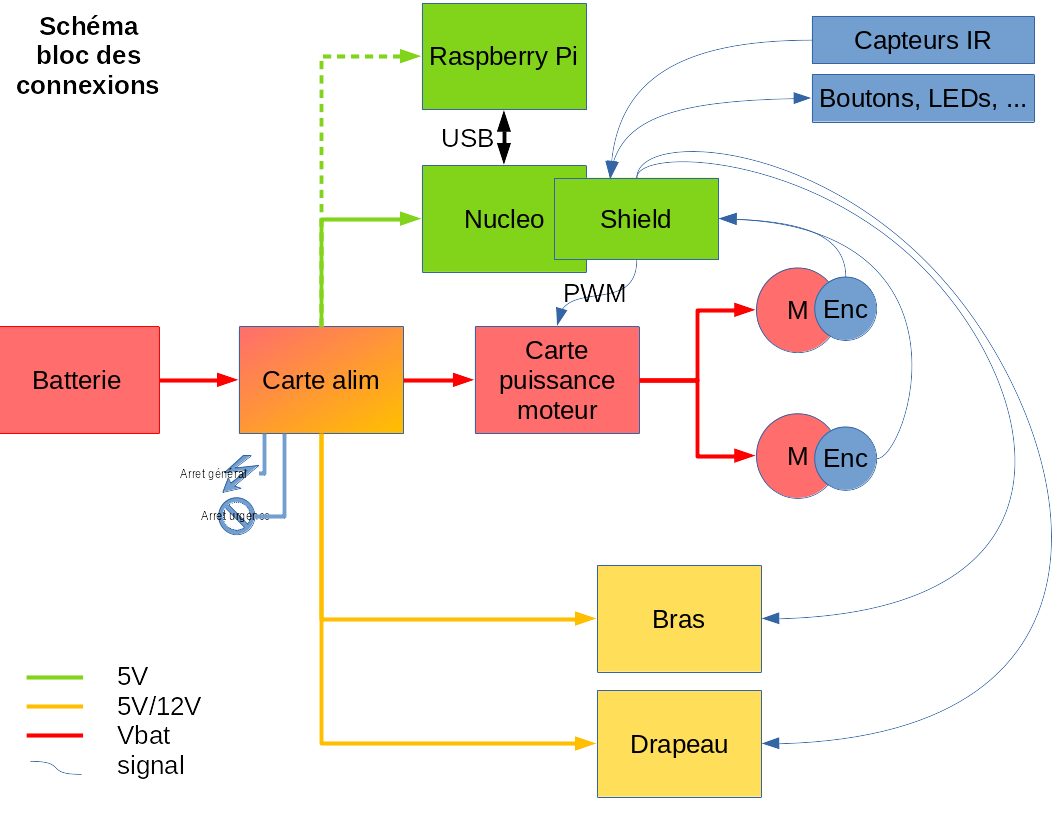
\includegraphics[scale=0.4]{schema_bloc_connexions.png}
  \caption{Schéma de principe de l'alimentation}
\end{figure}

\paragraph*{Point Puissance.}
Nous réutilisons les moteurs des 2A, le groupe travaillant dessus commence à
travailler.

\paragraph*{Point actionneur.}
Cnf tenaq pubfr à qver

\newpage
\section*{Jeudi 5 Décembre}
C'est bientôt Noël
\paragraph*{Point Table.}
Tous les éléments sont découpés et assemblés. Les manches à air sont montés et
la boussole est en cours de montage. Il restera les balises et au un écueil.

\paragraph*{Point Mécanique.}
L'étage du bas est modélisé, en attente de découpage. Nans a commandé les
profilés, la base pourra donc être montée sous peu.

\paragraph*{Point Phare.}
Le projet de l'ancien phare est correctement entéré. Marius est parti sur un
nouveau phare avec une base de bras robot comme ci contre.
\begin{figure}[H]
  \center
  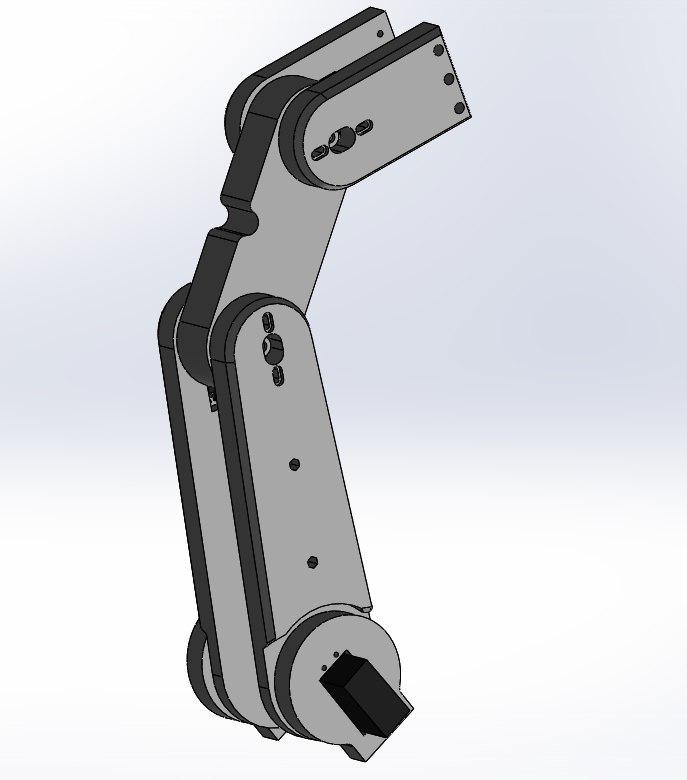
\includegraphics[scale=0.3]{phare.jpg}
  \caption{Version 2 du phare}
\end{figure}

\paragraph*{Point Asservissement + Info.}
Sébastien et Emile se battent avec le C++, Emile travaille sur les informations
renvoyées par les encodeurs pendant que Sébastien réflechit aux structures
qui permettrons au robot de correctement se déplacer.

\paragraph*{Point Alimentation.}
La carte d'alimentation avance bien, le travail de conception est en cours le
schéma de la carte d'alimentation sera disponible la semaine prochaine.

\paragraph*{Point Puissance.}
Y'vqér rfg q'nggraqer Znegva , cnepr dh'vy nvzr znatre qrf enqvngrhef nanybtvdhrf

\paragraph*{Point Actionneur.}
Les actionneurs sont au point morts pour l'instant, ce n'est pas l'urgence.


\part{Description des projets}
\chapter{Description générale de l'organisation}
\section{Arbres des tâches à réaliser par le robot}
\label{taches}
\HRule
\begin{center}
\begin{tikzpicture}
\tikzstyle{lien}=[->,>=stealth,rounded corners=20pt,thick]
\tikzset{individu/.style={draw,thick,fill=#1!25},
individu/.default={white}}
\node[individu=blue] (A) at (0,0) {\textsc{Se mouvoir}};
\node[individu] (A1) at (-7,-2) {Odométrie};
\node[individu] (A2) at (-3,-2) {Moteurs Maxon};
\node[individu] (A3) at (7,-2) {Asservissement};
\node[individu] (A3b) at (7,-4) {Encodeur};
\node[individu] (A4) at (3,-2) {\xout{Roue folle 2 roues motrices}};
\node[individu] (A5) at (3,-4) {2 roues motrice + patins};

\draw[lien] (A) -- (A1);
\draw[lien] (A) -- (A2);
\draw[lien] (A) -- (A3);
\draw[lien] (A) -- (A4);
\draw[lien] (A3) -- (A3b);
\draw[lien] (A4) -- (A5);


\end{tikzpicture}
\end{center}

\begin{center}
\begin{tikzpicture}
\tikzstyle{lien}=[->,>=stealth,rounded corners=20pt,thick]
\tikzset{individu/.style={draw,thick,fill=#1!25},
individu/.default={white}}
\node[individu=blue] (A) at (0,0) {\textsc{Mécanique générale}};
\node[individu] (A1) at (-3,-2) {Structure octogonale};
\node[individu] (A2) at (0,-2) {Profilés};
\node[individu] (A3) at (3,-2) {Etage rectangulaire};

\draw[lien] (A) -- (A1);
\draw[lien] (A) -- (A3);
\draw[lien] (A) -- (A2);

\end{tikzpicture}
\end{center}
\HRule
\begin{multicols}{2}
\begin{center}
\begin{tikzpicture}
\tikzstyle{lien}=[->,>=stealth,rounded corners=20pt,thick]
\tikzset{individu/.style={draw,thick,fill=#1!25},
individu/.default={white}}
\node[individu=red] (A) at (0,0) {\textsc{Détecter adversaire}};
\node[individu] (A1) at (0,-2) {Capteurs};
\node[individu] (A1a) at (-2,-4) {\xout{Ultrasons}};
\node[individu] (A1b) at (2,-4) {Infra rouge};

\draw[lien] (A) -- (A1);
\draw[lien] (A1) -- (A1a);
\draw[lien] (A1) -- (A1b);

\end{tikzpicture}
\end{center}
\columnbreak
\begin{center}
\begin{tikzpicture}
\tikzstyle{lien}=[->,>=stealth,rounded corners=20pt,thick]
\tikzset{individu/.style={draw,thick,fill=#1!25},
individu/.default={white}}
\node[individu=red] (A) at (0,0) {\textsc{Détecter Objet}};
\node[individu] (A1) at (-2,-2) {Couleur écocup};
\node[individu] (A1a) at (-2,-4) {Capteurs RGB};\node[individu] (A2) at (2,-2) {Pendant le ramassage};

\draw[lien] (A) -- (A1);
\draw[lien] (A1) -- (A1a);
\draw[lien] (A) -- (A2);
\draw (-3,0) -- (3,-4);
\draw (3,0) -- (-3,-4);


\end{tikzpicture}
\end{center}
\end{multicols}

\begin{multicols}{2}
\begin{center}
\begin{tikzpicture}
\tikzstyle{lien}=[->,>=stealth,rounded corners=20pt,thick]
\tikzset{individu/.style={draw,thick,fill=#1!25},
individu/.default={white}}
\node[individu=red] (A) at (0,0) {\textsc{Lire boussole}};
\node[individu] (A1) at (-2,-2) {Capteur};
\node[individu] (A1a) at (-2,-4) {Webcam};\node[individu] (A2) at (2,-2) {Balise sur le côté};

\draw[lien] (A) -- (A1);
\draw[lien] (A1) -- (A1a);
\draw[lien] (A) -- (A2);

\end{tikzpicture}
\end{center}
\columnbreak
\begin{center}
\begin{tikzpicture}
\tikzstyle{lien}=[->,>=stealth,rounded corners=20pt,thick]
\tikzset{individu/.style={draw,thick,fill=#1!25},
individu/.default={white}}
\node[individu=red] (A) at (0,0) {\textsc{Communication}};
\node[individu] (A1) at (-2,-2) {InfraRouge};;\node[individu] (A2) at (2,-2) {Bluetooth};

\draw[lien] (A) -- (A1);
\draw[lien] (A) -- (A2);

\end{tikzpicture}
\end{center}
\end{multicols}
\HRule

\begin{multicols}{2}
\begin{center}
\begin{tikzpicture}
\tikzstyle{lien}=[->,>=stealth,rounded corners=20pt,thick]
\tikzset{individu/.style={draw,thick,fill=#1!25},
individu/.default={white}}
\node[individu=green] (A) at (0,0) {\textsc{Elévation drapeau}};
\node[individu] (A1) at (-2,-2) {Timer};
\node[individu] (A2) at (2,-2) {Servomoteurs};

\draw[lien] (A) -- (A1);
\draw[lien] (A) -- (A2);

\end{tikzpicture}
\end{center}
\columnbreak
\begin{center}
\begin{tikzpicture}
\tikzstyle{lien}=[->,>=stealth,rounded corners=20pt,thick]
\tikzset{individu/.style={draw,thick,fill=#1!25},
individu/.default={white}}
\node[individu=green] (A) at (0,0) {\textsc{Manche à air}};
\node[individu] (A1) at (-2,-2) {Servomoteurs};
\node[individu] (A2) at (2,-2) {Coupler activation phare};

\draw[lien] (A) -- (A1);
\draw[lien] (A) -- (A2);

\end{tikzpicture}
\end{center}
\end{multicols}
\HRule

\begin{center}
\begin{tikzpicture}
\tikzstyle{lien}=[->,>=stealth,rounded corners=20pt,thick]
\tikzset{individu/.style={draw,thick,fill=#1!25},
individu/.default={white}}
\node[individu=gray] (A) at (0,0) {\textsc{Cartes}};
\node[individu] (A1) at (-4,-2) {Carte de puissance};
\node[individu] (A2) at (0,-2) {Carte de sécurité};
\node[individu] (A3) at (4,-2) {Carte d'alimentation};

\draw[lien] (A) -- (A1);
\draw[lien] (A) -- (A2);
\draw[lien] (A) -- (A3);


\end{tikzpicture}
\end{center}
\HRule

\begin{center}
\begin{tikzpicture}
\tikzstyle{lien}=[->,>=stealth,rounded corners=20pt,thick]
\tikzset{individu/.style={draw,thick,fill=#1!25},
individu/.default={white}}
\node[individu=orange] (A) at (0,0) {\textsc{Phare}};
\node[individu] (A1) at (-6,-2) {Elévation};
\node[individu] (A1a) at (-8,-4) {Bras robot};
\node[individu] (A1b) at (-4,-4) {\xout{Crémaillère}};
\node[individu] (A2) at (0,-2) {Activation};
\node[individu] (A2a) at (-1,-4) {\xout{Ddp}};
\node[individu] (A2b) at (1,-4) {Boutons};
\node[individu] (A3) at (6,-2) {Lumière};
\node[individu] (A3a) at (5,-4) {Ruban LED};
\node[individu] (A3b) at (7,-4) {\xout{Projo}};

\draw[lien] (A) -- (A1);
\draw[lien] (A1) -- (A1a);
\draw[lien] (A1) -- (A1b);
\draw[lien] (A) -- (A2);
\draw[lien] (A2) -- (A2a);
\draw[lien] (A2) -- (A2b);
\draw[lien] (A) -- (A3);
\draw[lien] (A3) -- (A3a);
\draw[lien] (A3) -- (A3b);


\end{tikzpicture}
\end{center}
\HRule

\newpage
\section{Répartition des tâches}
\label{repartition}
\HRule
\begin{center}
\begin{tikzpicture}
\tikzstyle{lien}=[->,>=stealth,rounded corners=20pt,thick]
\tikzset{individu/.style={draw,thick,fill=#1!25},
individu/.default={white}}
\node[individu=blue] (A) at (0,0) {\textsc{Se mouvoir} Carte puissance};
\node[individu] (A1) at (-3,-2) {Martin};
\node[individu] (A2) at (-1,-2) {\xout{Julien}};
\node[individu] (A3) at (1,-2) {Valentin};
\node[individu] (A4) at (3,-2) {Filipe};
 
\draw[lien] (A) -- (A1);
\draw[lien] (A) -- (A2);
\draw[lien] (A) -- (A3);
\draw[lien] (A) -- (A4);


\end{tikzpicture}
\end{center}
\begin{center}
\begin{tikzpicture}
\tikzstyle{lien}=[->,>=stealth,rounded corners=20pt,thick]
\tikzset{individu/.style={draw,thick,fill=#1!25},
individu/.default={white}}
\node[individu=blue] (A) at (0,0) {\textsc{Se mouvoir} Odométrie \& Asservissement};
\node[individu] (A1) at (-5,-2) {\xout{Raphaël}};
\node[individu] (A2) at (0,-2) {Clément};
\node[individu] (A3) at (5,-2) {SD};
\node[individu] (A4) at (-3,-2) {Emile};
\node[individu] (A5) at (3,-2) {Liam};

\draw[lien] (A) -- (A1);
\draw[lien] (A) -- (A2);
\draw[lien] (A) -- (A3);
\draw[lien] (A) -- (A4);
\draw[lien] (A) -- (A5);

\end{tikzpicture}
\end{center}

\begin{center}
\begin{tikzpicture}
\tikzstyle{lien}=[->,>=stealth,rounded corners=20pt,thick]
\tikzset{individu/.style={draw,thick,fill=#1!25},
individu/.default={white}}
\node[individu=blue] (A) at (0,0) {\textsc{Mécanique Générale}};
\node[individu] (A1) at (-4,-2) {Erwann};
\node[individu] (A2) at (-2,-2) {Filipe};
\node[individu] (A3) at (2,-2) {\xout{Valentin}};
\node[individu] (A4) at (4,-2) {\xout{Marion}};

\draw[lien] (A) -- (A1);
\draw[lien] (A) -- (A2);
\draw[lien] (A) -- (A3);
\draw[lien] (A) -- (A4);

\end{tikzpicture}
\end{center}
\HRule
\begin{multicols}{2}
\begin{center}
\begin{tikzpicture}
\tikzstyle{lien}=[->,>=stealth,rounded corners=20pt,thick]
\tikzset{individu/.style={draw,thick,fill=#1!25},
individu/.default={white}}
\node[individu=red] (A) at (0,0) {\textsc{Détecter Adversaire}};
\node[individu] (A1) at (-4,-2) {Martin};
\node[individu] (A2) at (-2,-2) {Liam};
\node[individu] (A3) at (2,-2) {\xout{Jeremy}};
\node[individu] (A4) at (4,-2) {\xout{Raphaël}};

\draw[lien] (A) -- (A1);
\draw[lien] (A) -- (A2);
\draw[lien] (A) -- (A3);
\draw[lien] (A) -- (A4);

\end{tikzpicture}
\end{center}
\columnbreak
\begin{center}
\begin{tikzpicture}
\tikzstyle{lien}=[->,>=stealth,rounded corners=20pt,thick]
\tikzset{individu/.style={draw,thick,fill=#1!25},
individu/.default={white}}
\node[individu=red] (A) at (0,0) {\textsc{Lire boussole}};
\node[individu] (A1) at (-2,-2) {Maxime};
\node[individu] (A2) at (0,-2) {Emile};
\node[individu] (A3) at (2,-2) {Léo};

\draw[lien] (A) -- (A1);
\draw[lien] (A) -- (A2);
\draw[lien] (A) -- (A3);

\end{tikzpicture}
\end{center}
\end{multicols}
\HRule
\begin{multicols}{2}
\begin{center}
\begin{tikzpicture}
\tikzstyle{lien}=[->,>=stealth,rounded corners=20pt,thick]
\tikzset{individu/.style={draw,thick,fill=#1!25},
individu/.default={white}}
\node[individu=green] (A) at (0,0) {\textsc{Elévation drapeau}};
\node[individu] (A1) at (-3,-2) {Filipe};
\node[individu] (A2) at (3,-2) {Erwann};
\node[individu] (A3) at (0,-2) {Valentin};

\draw[lien] (A) -- (A1);
\draw[lien] (A) -- (A2);
\draw[lien] (A) -- (A3);

\end{tikzpicture}
\end{center}
\columnbreak
\begin{center}
\begin{tikzpicture}
\tikzstyle{lien}=[->,>=stealth,rounded corners=20pt,thick]
\tikzset{individu/.style={draw,thick,fill=#1!25},
individu/.default={white}}
\node[individu=green] (A) at (0,0) {\textsc{Manche à air}};
\node[individu] (A1) at (-3,-2) {\xout{Jeremy}};
\node[individu] (A2) at (3,-2) {Marius};
\node[individu] (A3) at (0,-2) {Filipe};

\draw[lien] (A) -- (A1);
\draw[lien] (A) -- (A2);
\draw[lien] (A) -- (A3);

\end{tikzpicture}
\end{center}
\end{multicols}
\HRule

\begin{center}
\begin{tikzpicture}
\tikzstyle{lien}=[->,>=stealth,rounded corners=20pt,thick]
\tikzset{individu/.style={draw,thick,fill=#1!25},
individu/.default={white}}
\node[individu=orange] (A) at (0,0) {\textsc{Phare}};
\node[individu] (A1) at (-4,-2) {\xout{Marion}};
\node[individu] (A2) at (-2,-2) {\xout{Jeremy}};
\node[individu] (A3) at (2,-2) {Marius};
\node[individu] (A4) at (4,-2) {Erwann};

\draw[lien] (A) -- (A1);
\draw[lien] (A) -- (A2);
\draw[lien] (A) -- (A3);
\draw[lien] (A) -- (A4);

\end{tikzpicture}
\end{center}
\HRule

\begin{center}
\begin{tikzpicture}
\tikzstyle{lien}=[->,>=stealth,rounded corners=20pt,thick]
\tikzset{individu/.style={draw,thick,fill=#1!25},
individu/.default={white}}
\node[individu=gray] (A) at (0,0) {\textsc{Alimentation}};
\node[individu] (A1) at (-3,-2) {Julien};
\node[individu] (A2) at (-0,-2) {Ptit Lu};
\node[individu] (A3) at (3,-2) {Yohann};
\node[individu] (A4) at (5,-2) {\xout{Théo}};
\node[individu] (A5) at (-5,-2) {Léo};

\draw[lien] (A) -- (A1);
\draw[lien] (A) -- (A2);
\draw[lien] (A) -- (A3);
\draw[lien] (A) -- (A4);
\draw[lien] (A) -- (A5);

\end{tikzpicture}
\end{center}
\HRule

\section{Points pour la coupe}
\begin{center}
\begin{tikzpicture}
\tikzstyle{lien}=[->,>=stealth,rounded corners=20pt,thick]
\tikzset{individu/.style={draw,thick,fill=#1!25},
individu/.default={white}}
\node[individu=blue] (A) at (0,0 ){\textsc{Bouées}};
\node[individu] (A1) at (5,2){4 pour l'équipe à proximité du ports};
\node[individu] (A2) at (5,1){8 communs directement sur la table};
\node[individu] (A3) at (5,-1){6 pour l'équipe dans un ecceuil};
\node[individu] (A4) at (5,-2){12 communs dans des ecceuils};


\draw[lien] (A) --(0,2)-- (A1);
\draw[lien] (A) --(0,1)-- (A2);
\draw[lien] (A) --(0,-1)-- (A3);
\draw[lien] (A) --(0,-2)-- (A4);

\node[individu] (A5) at (-5,1){1 points par bouée valide};
\node[individu] (A6) at (-5,0){1 sup si la bouée est sur le bon chenal};
\node[individu] (A7) at (-5,-1){2 points par paire de bouée};


\draw[lien] (A) --(0,1)-- (A5);
\draw[lien] (A) -- (A6);
\draw[lien] (A) --(0,-1)-- (A7);

\tikzstyle{lien}=[->,>=stealth,rounded corners=20pt,thick]
\tikzset{individu/.style={draw,thick,fill=#1!25},
individu/.default={white}}
\node[individu=red] (B) at (0,-5 ){\textsc{Manche à air}};
\node[individu] (B1) at (5,-5){2 manche à airs au Sud du port};
\draw[lien] (B) -- (B1);


\node[individu] (B5) at (-5,-4){5 pour 1 manche};
\node[individu] (B6) at (-5,-6){15 pour 2 manches};


\draw[lien] (B) --(0,-4)-- (B5);
\draw[lien] (B) -- (0,-6) -- (B6);

\tikzstyle{lien}=[->,>=stealth,rounded corners=20pt,thick]
\tikzset{individu/.style={draw,thick,fill=#1!25},
individu/.default={white}}
\node[individu=green] (C) at (0,-10 ){\textsc{Allumer le phare}};
\node[individu] (C1) at (5,-10){1 phare au nord du port};
\draw[lien] (C) -- (C1);


\node[individu] (C5) at (-5,-9){2 pour poser le phare};
\node[individu] (C6) at (-5,-10){3 pour le déclancher};
\node[individu] (C7) at (-5,-11){10 pour activation correcte};


\draw[lien] (C) --(0,-9)-- (C5);
\draw[lien] (C) -- (0,-11) -- (C7);
\draw[lien] (C) -- (C6);

\node[individu=yellow] (D) at (0,-15 ){\textsc{Retourner au port}};
\node[individu] (D1) at (5,-15){Sur les largeurs de la table};
\draw[lien] (D) -- (D1);


\node[individu] (D5) at (-5,-13){1 robot 10 dans la bonne zone};
\node[individu] (D6) at (-5,-14){1 robot 5 dans la mauvaise zone};
\node[individu] (D7) at (-5,-16){2 robots 10 dans la bonne zone};
\node[individu] (D8) at (-5,-17){2 robots 5 dans la mauvaise zone};
\node[individu] (D9) at (-5,-18){2 robots 5 1 dans la bonne zone};
\node[individu] (D10) at (-5,-19){2 robots 5 dans des zones différentes};


\draw[lien] (D) --(0,-13)-- (D5);
\draw[lien] (D) --(0,-14)-- (D6);
\draw[lien] (D) -- (0,-16) -- (D7);
\draw[lien] (D) -- (0,-17) -- (D8);
\draw[lien] (D) -- (0,-18) -- (D9);
\draw[lien] (D) -- (0,-19) -- (D10);
\end{tikzpicture}
\end{center}

\chapter{Mécanique}
\section{Mécanique générale du robot}
\section{Actionneurs}

\chapter{Electronique}
\section{Alimentation}
\section{Puissance}
\section{Actionneur}

\chapter{Informatique}
\section{Asservissement}
\section{Stratégie}

\newpage
\end{spacing}
\end{document}
